
% Options for packages loaded elsewhere
\PassOptionsToPackage{unicode}{hyperref}
\PassOptionsToPackage{hyphens}{url}
%
\documentclass[
  ignorenonframetext,
]{beamer}
\usepackage{pgfpages}
\setbeamertemplate{caption}[numbered]
\setbeamertemplate{caption label separator}{: }
\setbeamercolor{caption name}{fg=normal text.fg}
\beamertemplatenavigationsymbolsempty
% Prevent slide breaks in the middle of a paragraph
\widowpenalties 1 10000
\raggedbottom
\setbeamertemplate{part page}{
  \centering
  \begin{beamercolorbox}[sep=16pt,center]{part title}
    \usebeamerfont{part title}\insertpart\par
  \end{beamercolorbox}
}
\setbeamertemplate{section page}{
  \centering
  \begin{beamercolorbox}[sep=12pt,center]{part title}
    \usebeamerfont{section title}\insertsection\par
  \end{beamercolorbox}
}
\setbeamertemplate{subsection page}{
  \centering
  \begin{beamercolorbox}[sep=8pt,center]{part title}
    \usebeamerfont{subsection title}\insertsubsection\par
  \end{beamercolorbox}
}
\AtBeginPart{
  \frame{\partpage}
}
\AtBeginSection{
  \ifbibliography
  \else
    \frame{\sectionpage}
  \fi
}
\AtBeginSubsection{
  \frame{\subsectionpage}
}
\usepackage{lmodern}
\usepackage{amssymb,amsmath}
\usepackage{ifxetex,ifluatex}
\ifnum 0\ifxetex 1\fi\ifluatex 1\fi=0 % if pdftex
  \usepackage[T1]{fontenc}
  \usepackage[utf8]{inputenc}
  \usepackage{textcomp} % provide euro and other symbols
\else % if luatex or xetex
  \usepackage{unicode-math}
  \defaultfontfeatures{Scale=MatchLowercase}
  \defaultfontfeatures[\rmfamily]{Ligatures=TeX,Scale=1}
\fi
\usetheme[]{Madrid}
% Use upquote if available, for straight quotes in verbatim environments
\IfFileExists{upquote.sty}{\usepackage{upquote}}{}
\IfFileExists{microtype.sty}{% use microtype if available
  \usepackage[]{microtype}
  \UseMicrotypeSet[protrusion]{basicmath} % disable protrusion for tt fonts
}{}
\makeatletter
\@ifundefined{KOMAClassName}{% if non-KOMA class
  \IfFileExists{parskip.sty}{%
    \usepackage{parskip}
  }{% else
    \setlength{\parindent}{0pt}
    \setlength{\parskip}{6pt plus 2pt minus 1pt}}
}{% if KOMA class
  \KOMAoptions{parskip=half}}
\makeatother
\usepackage{xcolor}
\IfFileExists{xurl.sty}{\usepackage{xurl}}{} % add URL line breaks if available
\IfFileExists{bookmark.sty}{\usepackage{bookmark}}{\usepackage{hyperref}}
\hypersetup{
  pdftitle={Methods for Selection Bias in the UK Biobank},
  pdfauthor={Valerie Bradley},
  hidelinks,
  pdfcreator={LaTeX via pandoc}}
\urlstyle{same} % disable monospaced font for URLs
\newif\ifbibliography
\usepackage{graphicx,grffile}
\makeatletter
\def\maxwidth{\ifdim\Gin@nat@width>\linewidth\linewidth\else\Gin@nat@width\fi}
\def\maxheight{\ifdim\Gin@nat@height>\textheight\textheight\else\Gin@nat@height\fi}
\makeatother
% Scale images if necessary, so that they will not overflow the page
% margins by default, and it is still possible to overwrite the defaults
% using explicit options in \includegraphics[width, height, ...]{}
\setkeys{Gin}{width=\maxwidth,height=\maxheight,keepaspectratio}
% Set default figure placement to htbp
\makeatletter
\def\fps@figure{htbp}
\makeatother
\setlength{\emergencystretch}{3em} % prevent overfull lines
\providecommand{\tightlist}{%
  \setlength{\itemsep}{0pt}\setlength{\parskip}{0pt}}
\setcounter{secnumdepth}{-\maxdimen} % remove section numbering
%\setbeamertemplate{navigation symbols}{}
%ß\setbeamertemplate{footline}[frame number]{}

\usepackage{tikz}
\usepackage{colortbl}
\usepackage[]{algorithm2e}
\usepackage{pifont}
\usepackage{amssymb}

\usetikzlibrary{shapes,decorations,arrows,calc,arrows.meta,fit,positioning}
\tikzset{
	-Latex,auto,node distance =1 cm and 1 cm,semithick,
	state/.style ={ellipse, draw, minimum width = 3 cm},
	point/.style = {circle, draw, inner sep=0.04cm,fill,node contents={}},
	bidirected/.style={Latex-Latex,dashed},
	el/.style = {inner sep=2pt, align=left, sloped}
}

\newcommand\ci{\perp\!\!\!\perp}

%\title[Methods for Selection Bias in the UK Biobank]{Methods for Selection Bias in UKB}
\institute[University of Oxford]{University of Oxford, Department of Statistics}

\titlegraphic{
	\vspace{1cm}
	\includegraphics[width=3cm]{/Users/valeriebradley/Documents/Oxford/logos/ox_small_cmyk_pos_rect.png}
}

%\definecolor{oxfordblue}{rgb}{0.267, 0.412, 0.49}
\definecolor{oxfordblue}{rgb}{0, 0.129, 0.278}
\definecolor{oxfordlightblue}{RGB}{25, 56, 87}
\definecolor{oxfordred}{RGB}{186, 12, 47}
\definecolor{oxfordgreen}{RGB}{15,115,97}
\usecolortheme[named=oxfordblue]{structure}


\defbeamertemplate{section page}{mine}[1][]{%
	\begin{centering}
		{\usebeamerfont{section name}\usebeamercolor[fg]{section name}#1}
		\vskip1em\par
		\begin{beamercolorbox}[sep=12pt,center]{part title}
			\usebeamerfont{section title}\insertsection\par
		\end{beamercolorbox}
	\end{centering}
}


\setbeamertemplate{section page}[mine]

\title{Methods for Selection Bias in the UK Biobank}
\author{Valerie Bradley}
\date{15 October 2019}

\begin{document}
\frame{\titlepage}

\begin{frame}
  \tableofcontents[hideallsubsections]
\end{frame}
\hypertarget{unrepresentativeness-in-the-uk-biobank}{%
\section{Unrepresentativeness in the UK
Biobank}\label{unrepresentativeness-in-the-uk-biobank}}

\begin{frame}{About the data}
\protect\hypertarget{about-the-data}{}

\textbf{UK Biobank}

\begin{itemize}
\tightlist
\item
  \textbf{Goal}: Study exposures and outcomes that affect aging
  populations
\item
  500,000+ participants aged 40-70 when recruited between 2006 and 2010
\item
  \emph{Not representative of the UK general population} (Fry et al.
  2017)
\end{itemize}

\textbf{UK Biobank imaging cohort}

\begin{itemize}
\tightlist
\item
  Subset of UKB participants, undergo additional imaging exams
\item
  21,407 complete, valid T1 structural MRIs (4\% of UKB)
\end{itemize}

\textbf{\href{https://digital.nhs.uk/data-and-information/publications/statistical/health-survey-for-england/health-survey-for-england-2016}{2016
Health Survey for England}}

\begin{itemize}
\tightlist
\item
  Designed to estimate prevalence of health outcomes (e.g.~smoking,
  obesity, high blood pressure)
\item
  2016 survey contains 10,067 respondents, 4,318 aged 45-80
\end{itemize}

\end{frame}

\begin{frame}{Quantifying unrepresentativeness of the UKB}
\protect\hypertarget{quantifying-unrepresentativeness-of-the-ukb}{}

\begin{center}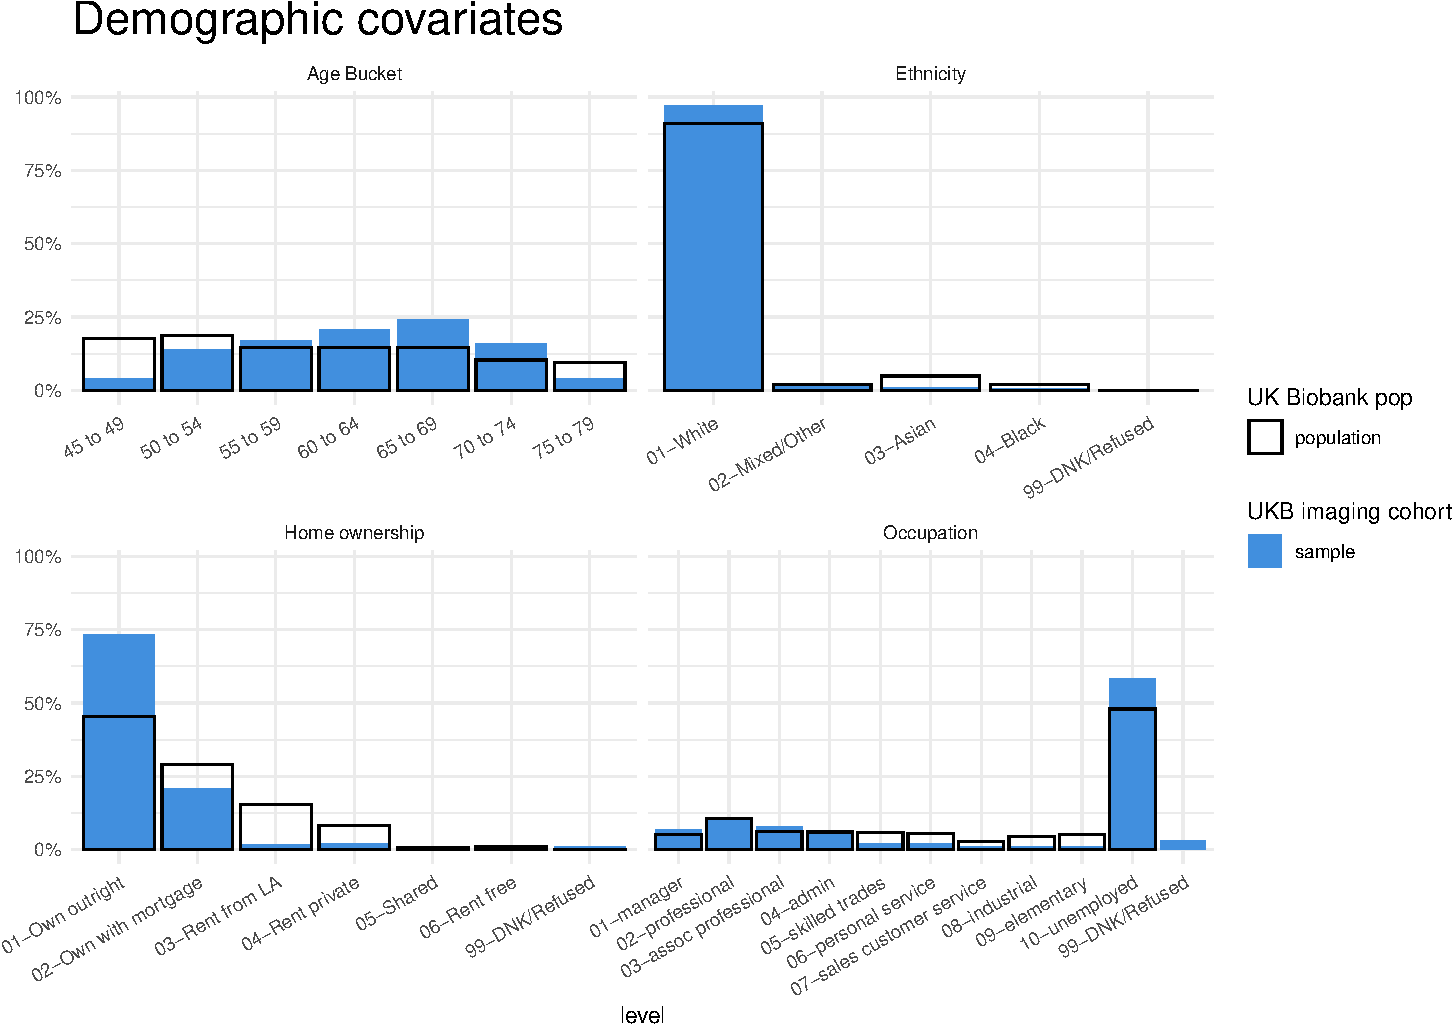
\includegraphics[width=0.95\linewidth]{fmrib-deck-20191002_files/figure-beamer/plot-selection-bias-demos-1} \end{center}

\end{frame}

\begin{frame}{Quantifying unrepresentativeness of the UKB}
\protect\hypertarget{quantifying-unrepresentativeness-of-the-ukb-1}{}

\begin{center}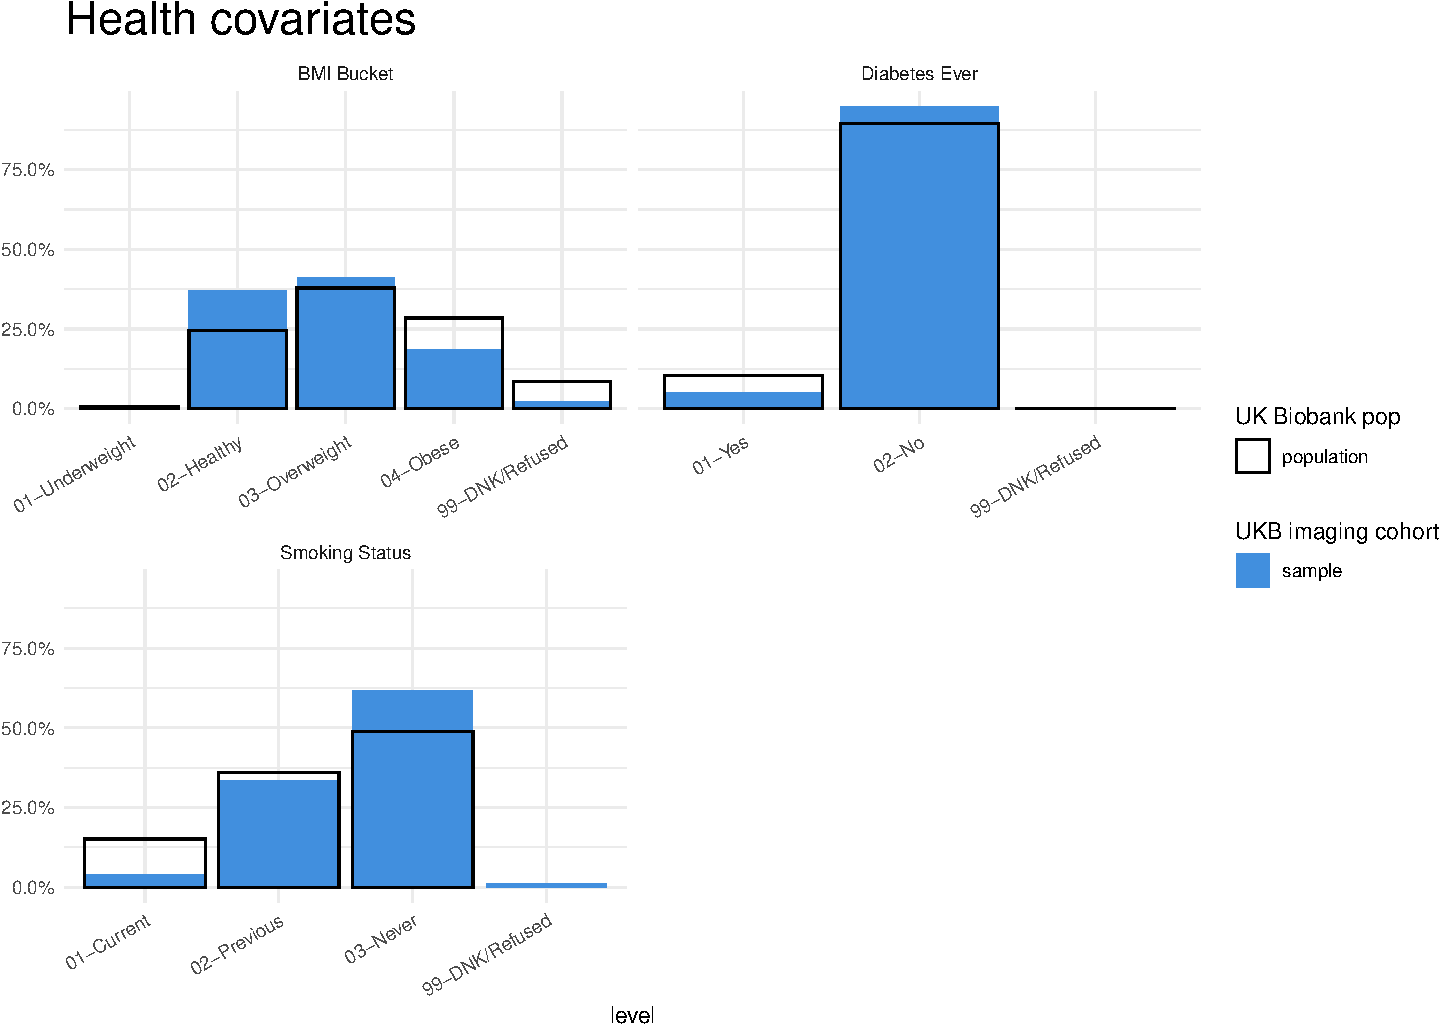
\includegraphics[width=0.95\linewidth]{fmrib-deck-20191002_files/figure-beamer/plot-selection-bias-health-1} \end{center}

\end{frame}

\hypertarget{why-is-unrepresentativeness-a-problem}{%
\section{Why is unrepresentativeness a
problem?}\label{why-is-unrepresentativeness-a-problem}}

\begin{frame}{Quick note on structural causal models (SCMs)}
\protect\hypertarget{quick-note-on-structural-causal-models-scms}{}

SCMs use directed acyclic graphs (DAGs) as ``a mathematical language for
integrating statistical and subject-matter information," specifically
information about dependence structures (Pearl 1995)

\begin{itemize}
\tightlist
\item
  \textbf{nodes} represent \emph{physical mechanisms}
\item
  \textbf{edges} represent \emph{direct causal pathways}
\end{itemize}

\begin{figure}
\centering
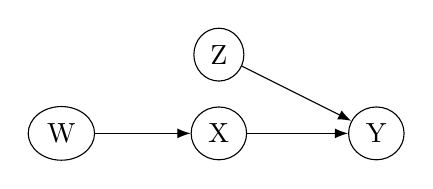
\begin{tikzpicture}
    \node[state, minimum width=0.5cm] (w) at (-2,0) {W};
    \node[state, minimum width=0.5cm] (x) at (0,0) {X};
    \node[state, minimum width=0.5cm] (y) at (2,0) {Y};
    \node[state, minimum width=0.5cm] (z) at (0,1) {Z};
    
        \path (x) edge (y);
    \path (w) edge (x);
    \path (z) edge (y); 
\end{tikzpicture}
\end{figure}

Things we can say:

\begin{itemize}
\tightlist
\item
  there is a \emph{direct} causal pathway from \(X\) to \(Y\)
\item
  there is an \emph{indirect} causal pathway from \(W\) to \(Y\)
\item
  \(X\) \emph{d-separates} \(W\) and \(Y\), such that \(W \ci Y | X\)
\end{itemize}

\end{frame}

\begin{frame}{SCM Example}
\protect\hypertarget{scm-example}{}

\begin{figure}
\centering
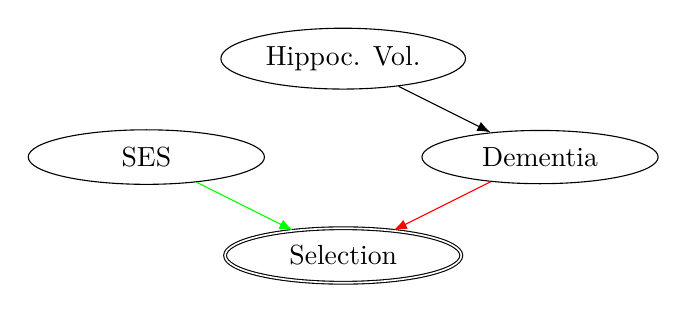
\begin{tikzpicture}
    \node[state] (x) at (0,1.25) {SES};
    \node[state, double] (s) at (2.5,0) {Selection};
    
    \node[state] (y) at (2.5,2.5) {Hippoc. Vol.};
    \node[state] (z) at (5,1.25) {Dementia};

    \path (x) edge[green] (s);
    \path (y) edge (z);
    \path (z) edge[red] (s);
    %\path [dashed, >=latex, style={<->}, fill=oxfordred, color=oxfordred] (x) edge [bend left=10]  (z);
    
    \end{tikzpicture}
\end{figure}

\begin{itemize}
\tightlist
\item
  SES and participation in UKB are \textcolor{green}{positively}
  correlated
\item
  Dementia and participation are \textcolor{red}{negatively} correlated
\item
  No causal relationship between SES and hippocampal volume (no edge)
\end{itemize}

Are SES and Dementia independent?

\end{frame}

\begin{frame}{Collider bias}
\protect\hypertarget{collider-bias}{}

\begin{figure}
\centering
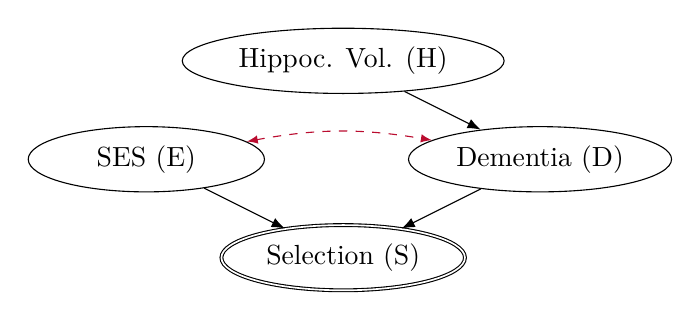
\begin{tikzpicture}
    \node[state] (x) at (0,1.25) {SES (E)};
    \node[state, double] (s) at (2.5,0) {Selection (S)};
    
    \node[state] (y) at (2.5,2.5) {Hippoc. Vol. (H)};
    \node[state] (z) at (5,1.25) {Dementia (D)};

    \path (x) edge (s);
    \path (y) edge (z);
    \path (z) edge (s);
    \path [dashed, >=latex, style={<->}, fill=oxfordred, color=oxfordred] (x) edge [bend left=10]  (z);
    
    \end{tikzpicture}
\end{figure}

\textbf{Collider bias}: ``When two variables independently influence a
third variable, and that third variable is conditioned upon'' (Munafò et
al. 2018)

Opens a \emph{backdoor path} (spurious association) between E and H.

\begin{itemize}
\tightlist
\item
  Want to know \(\text{P(H|E)}\)
\item
  But only observe \(\text{P}(H | E, S = 1)\)
\item
  And, because \(H\), \(E\) are \emph{not} independent of \(S\), those
  are not the same
\end{itemize}

\end{frame}

\begin{frame}{Collider bias example}
\protect\hypertarget{collider-bias-example}{}

Day et al. (2016): GWAS using 142,630 observations from the UKB, induced
strong collider bias

\begin{figure}
\centering
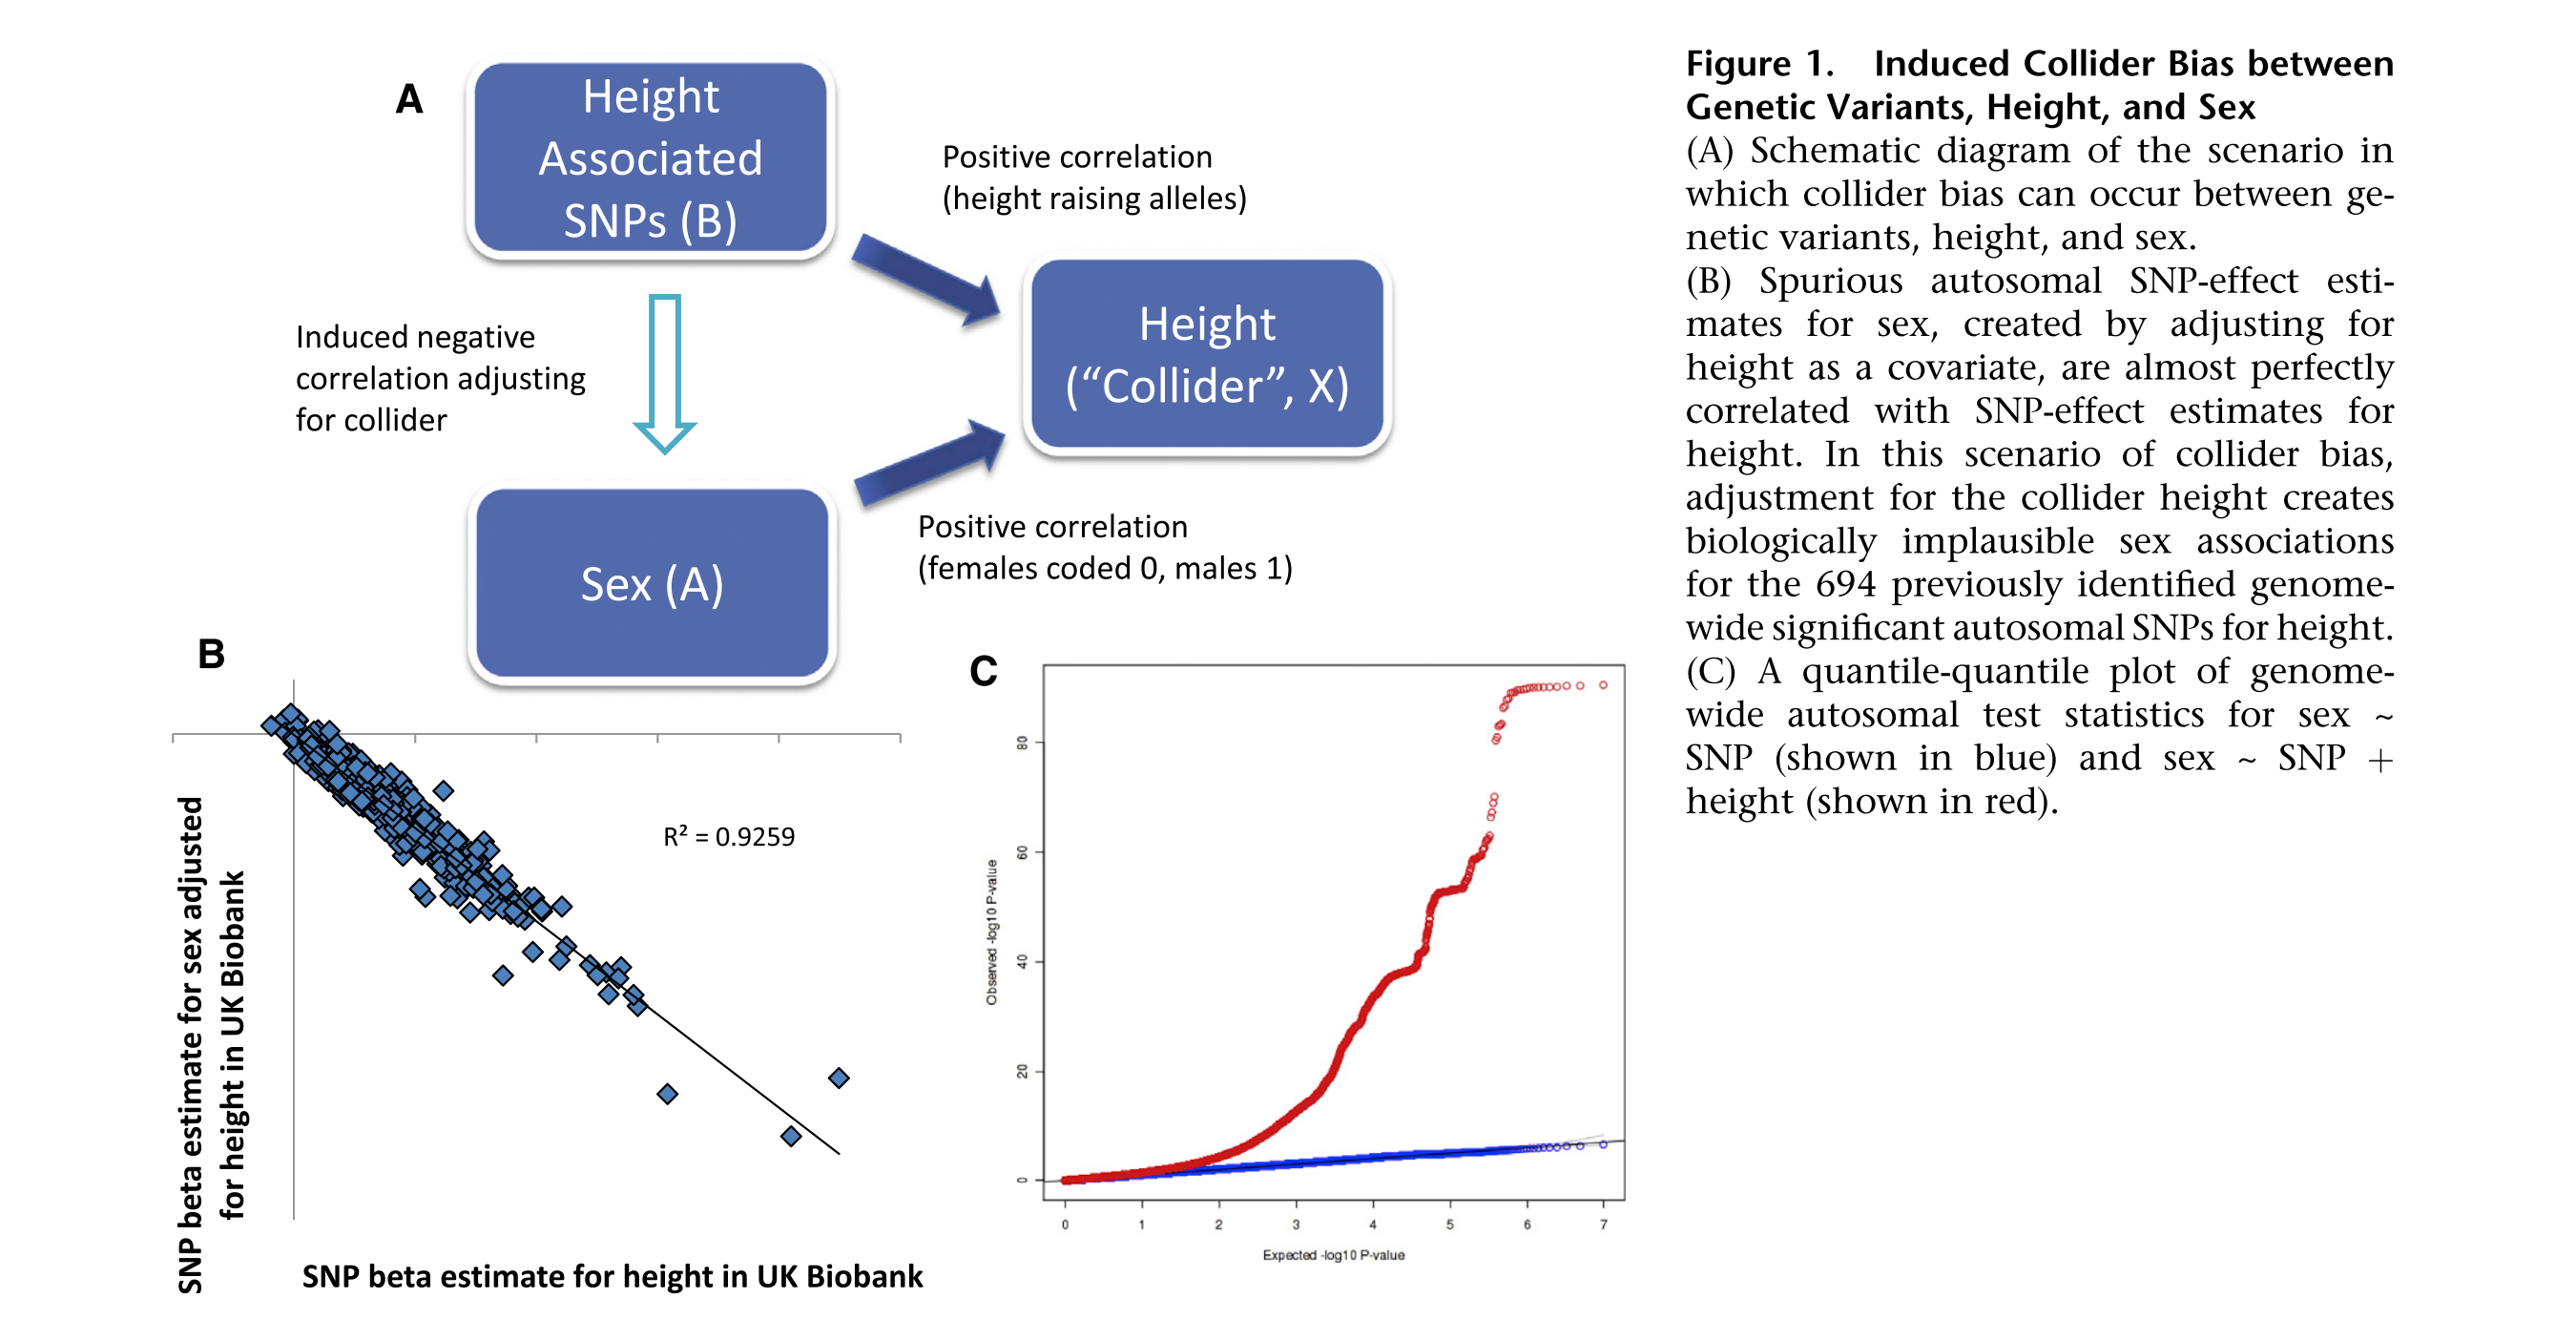
\includegraphics[width=\textwidth]{collider_bias_example.png}
\end{figure}

\end{frame}

\hypertarget{can-we-recover-from-selection-bias}{%
\section{Can we recover from selection
bias?}\label{can-we-recover-from-selection-bias}}

\begin{frame}{Formal conditions for recovery}
\protect\hypertarget{formal-conditions-for-recovery}{}

Consider the \emph{association} between \(X\) and \(Y\),
\(\text{P}(y|x)\)

We can recover from selection bias \textbf{if and only if}
\(\text{P}(y|x)\) can be written in terms of the quantities observed
under selection; use \emph{auxilary variables} \(\mathbf{Z}\)

\begin{itemize}
\tightlist
\item
  if \(Y \ci S | \{\mathbf{Z}, X\}\), then
  \[\text{P}(y|x) = \sum_\mathbf{z} \text{P}(y|x, \mathbf{z}, S=1)\text{P}(\mathbf{z}|x)\]
\item
  If \(\{Y \cup X\} \ci S | \mathbf{Z}\), then
  \[\text{P}(y|x) = \sum_\mathbf{z} \text{P}(y|x, \mathbf{z}, S=1)\text{P}(\mathbf{z})\]
\end{itemize}

\textbf{The key:} conditioning on \(\mathbf{Z}\) (and maybe \(X\)) makes
\(Y\) \emph{conditionally independent of selection} \(S\)

\(\text{P}(\mathbf{z})\) and \(\text{P}(\mathbf{z}|x)\) are population
distributions

\end{frame}

\begin{frame}{Example}
\protect\hypertarget{example}{}

Back to our example\ldots{}

\begin{figure}
\centering
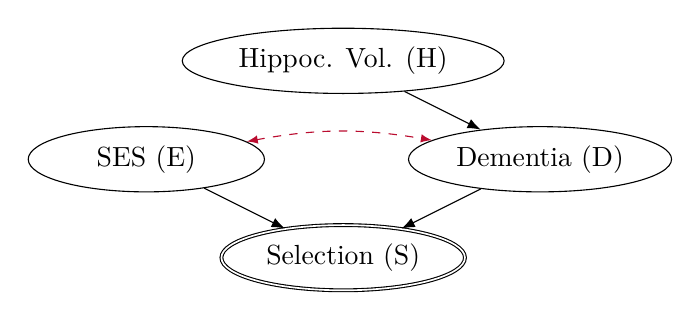
\begin{tikzpicture}
    \node[state] (x) at (0,1.25) {SES (E)};
    \node[state, double] (s) at (2.5,0) {Selection (S)};
    
    \node[state] (y) at (2.5,2.5) {Hippoc. Vol. (H)};
    \node[state] (z) at (5,1.25) {Dementia (D)};

    \path (x) edge (s);
    \path (y) edge (z);
    \path (z) edge (s);
    \path [dashed, >=latex, style={<->}, fill=oxfordred, color=oxfordred] (x) edge [bend left=10]  (z);
    
    \end{tikzpicture}
\end{figure}

\begin{itemize}
\item[\rlap{\raisebox{0.3ex}{\hspace{0.4ex}\scriptsize \textcolor{red}{\ding{56}}}}$\square$] \(\{H \cup E\} \ci S | D\)
\item[\rlap{\raisebox{0.3ex}{\hspace{0.4ex}\tiny \textcolor{green}{\ding{52}}}}$\square$] \(H \ci S | D, E\)
\end{itemize}

So, can only recover \(\text{P}(H | E)\) as
\[\text{P}(H | E) = \sum_D\text{P}(H | E, D, S = 1) P (D|E)\] \emph{as
long as we observe} \(\text{P}(D | E)\)

\end{frame}

\begin{frame}{Problems}
\protect\hypertarget{problems}{}

\begin{enumerate}
\item
  Must assume we have correctly represented the dependence structures
  (and have correctly identified all necessary elements of
  \(\mathbf{Z}\)). This is \textbf{hard} to do in practice.
\item
  Don't always observe \(\text{P}(\mathbf{Z} | X)\) or
  \(\text{P}(\mathbf{Z})\) in full. \emph{Can we estimate it?}
\item
  Can only condition on a limited number of discrete variables
  \(\mathbf{Z}\) before this breaks down. \emph{What happens when an
  element of \(\mathbf{Z}\) is continuous?}
\end{enumerate}

\end{frame}

\hypertarget{methods-for-recovering-from-selection-bias}{%
\section{Methods for recovering from selection
bias}\label{methods-for-recovering-from-selection-bias}}

\begin{frame}{Two main methods for recovery}
\protect\hypertarget{two-main-methods-for-recovery}{}

Classes of methods for estimating effects, associations, prevalence in
the presence of selection bias:

\begin{itemize}
\tightlist
\item
  \textbf{Inverse probability weighting (IPW)}: weight each observed
  unit by the inverse of the probability of selection,
  \(w_i \propto 1/\text{P}(S = 1 | \mathbf{Z}_i)\)

  \begin{itemize}
  \tightlist
  \item
    \textcolor{oxfordgreen}{pro}: weights are independent of \(Y\) and
    \(X\)
  \item
    \textcolor{oxfordred}{con}: not always clear how to incorporate into
    estimators
  \item
    \textcolor{oxfordred}{con}: hard to correctly estimate standard
    errors of weighted estimators \vspace{0.25cm}
  \end{itemize}
\item
  \textbf{Regression methods}: directly model the outcome of interest
  \(\text{P}(Y|X)\), accounting for confounders/auxiliary variables

  \begin{itemize}
  \tightlist
  \item
    \textcolor{oxfordred}{con}: have to estimate separate model for each
    outcome
  \end{itemize}
\end{itemize}

\end{frame}

\begin{frame}{Inverse probability weighting (IPW)}
\protect\hypertarget{inverse-probability-weighting-ipw}{}

Can be derived exactly from (causal) recovery conditions (Correa, Tian,
and Bareinboim 2018): \begin{align}
\text{P}(\mathbf{y}|do(\mathbf{x})) &= \sum_\mathbf{Z} \text{P}(\mathbf{y}|\mathbf{x}, \mathbf{z}, S=1)\text{P}(\mathbf{z}\setminus\mathbf{z^T}|\mathbf{z^T}, S = 1)\text{P}(\mathbf{z^T})\\
&= \sum_\mathbf{Z} \frac{\textcolor{oxfordred}{\text{P}(\mathbf{y}, \mathbf{x}, \mathbf{z} | S = 1)}}{\textcolor{oxfordlightblue}{\text{P}(\mathbf{x}| \mathbf{z}, S = 1)}} \textcolor{oxfordgreen}{\frac{\text{P}(S = 1)}{\text{P}(S = 1 | \mathbf{z^T})}} \label{eq:IPSW}
\end{align}

\begin{itemize}
\tightlist
\item
  \(\textcolor{oxfordred}{\text{P}(\mathbf{y}, \mathbf{x}, \mathbf{z} | S = 1)}\),
  joint distribution of \(\mathbf{Y}\), \(\mathbf{X}\) and
  \(\mathbf{Z}\) under selection bias
\item
  \(\textcolor{oxfordlightblue}{\text{P}(\mathbf{x}| \mathbf{z}, S = 1)}\),
  the probability of treatment given covariates in the selection-biased
  sample data

  \begin{itemize}
  \tightlist
  \item
    related to the \emph{propensity score} \(\text{P}(X|\mathbf{Z})\)
  \end{itemize}
\item
  \(\textcolor{oxfordgreen}{\text{P}(S = 1)/\text{P}(S = 1 | \mathbf{z^T})}\),
  the \textit{inverse probability-of-selection weight}
\end{itemize}

\textbf{But how should we estimate \(\text{P}(S = 1 | \mathbf{Z})\)?}

\end{frame}

\begin{frame}{Estimating \(\text{P}(S = 1 | \mathbf{Z})\)}
\protect\hypertarget{estimating-textps-1-mathbfz}{}

Things to think about when comparing methods for estimating
\(\text{P}(S = 1 | \mathbf{Z})\):

\begin{enumerate}
\item
  Weighted \textbf{marginal distribution} of \(\mathbf{Z}\) should match
  that of the population
\item
  Avoid extreme weights that inflate the \textbf{variance} of estimators
  (have to account for the additional uncertainty of weights)
\item
  \textbf{Computational complexity} of the method
\item
  How well does the method account for interactions between elements of
  \(\mathbf{Z}\)
\end{enumerate}

\end{frame}

\begin{frame}{Methods: summary}
\protect\hypertarget{methods-summary}{}

Classic weighting methods:

\begin{enumerate}
\tightlist
\item
  \emph{Post-stratification}: adjust to the joint distribution of
  \(\mathbf{Z}\)
\item
  \emph{Raking}: iteratively adjust the marginal distributions of
  elements in \(\mathbf{Z}\)
\item
  \emph{Calibration}: raking, but with continuous variables as well as
  discrete variables
\end{enumerate}

Less-common methods:

\begin{enumerate}
\setcounter{enumi}{3}
\tightlist
\item
  \emph{Logit}: estimate the probability of selection directly
\item
  \emph{LASSO}: use a LASSO to select variables and interactions for
  raking
\end{enumerate}

New method:

\begin{enumerate}
\setcounter{enumi}{5}
\tightlist
\item
  \emph{BART + raking}: use a Bayesian Additive Regression Tree (BART)
  to estimate the probability of selection, then rake such that key
  marginal distributions match those of the population
\end{enumerate}

\end{frame}

\hypertarget{application-to-the-uk-biobank}{%
\section{Application to the UK
Biobank}\label{application-to-the-uk-biobank}}

\begin{frame}{Simulation overview}
\protect\hypertarget{simulation-overview}{}

\begin{enumerate}
\tightlist
\item
  Generate a probability of missingness \(p_i\) for all 21,407 imaging
  subjects in the UKB

  \begin{itemize}
  \tightlist
  \item
    \(p_i\) depends on covariates that we know to be related to brain
    volume (mainly age) so that samples are biased
  \end{itemize}
\item
  For sample sizes in
  \(n_{sim} = 21,407 \times (0.01, 0.02, 0.04,0.05,0.075, 0.1, 0.25)\):

  \begin{enumerate}
  \tightlist
  \item
    Draw sample of size \(n_{sim}\) from imaging cohort with probability
    proportional to \(p_i\)
  \item
    Weight sample to \(P(\mathbf{Z})\) defined by UKB imaging cohort
    using each of 6 methods
  \item
    Perform steps 2.1-2.2 1000 times
  \end{enumerate}
\end{enumerate}

\end{frame}

\begin{frame}{Simulation overview}
\protect\hypertarget{simulation-overview-1}{}

Evaluate methods based on:

\begin{itemize}
\item
  \textbf{design effect}: measures the decrease in effective sample size
  (ESS) from weighting
  \[\text{deff}(\mathbf{w}) = 1 + \text{Var}(\mathbf{w})\]
  \[ESS = \frac{n}{\text{deff}(\mathbf{w})}\]
\item
  \textbf{Absolute bias} of estimated average total brain volume
\end{itemize}

\[\text{bias} = |\bar{Y}^w - \mu|\]
\[\bar{Y}^w = \frac{1}{n_{sim}}\sum_{i = 1}^{n_{sim}} Y_i \hat{w}_i\]

\end{frame}

\begin{frame}{Simulation results}
\protect\hypertarget{simulation-results}{}

\begin{figure}
\centering
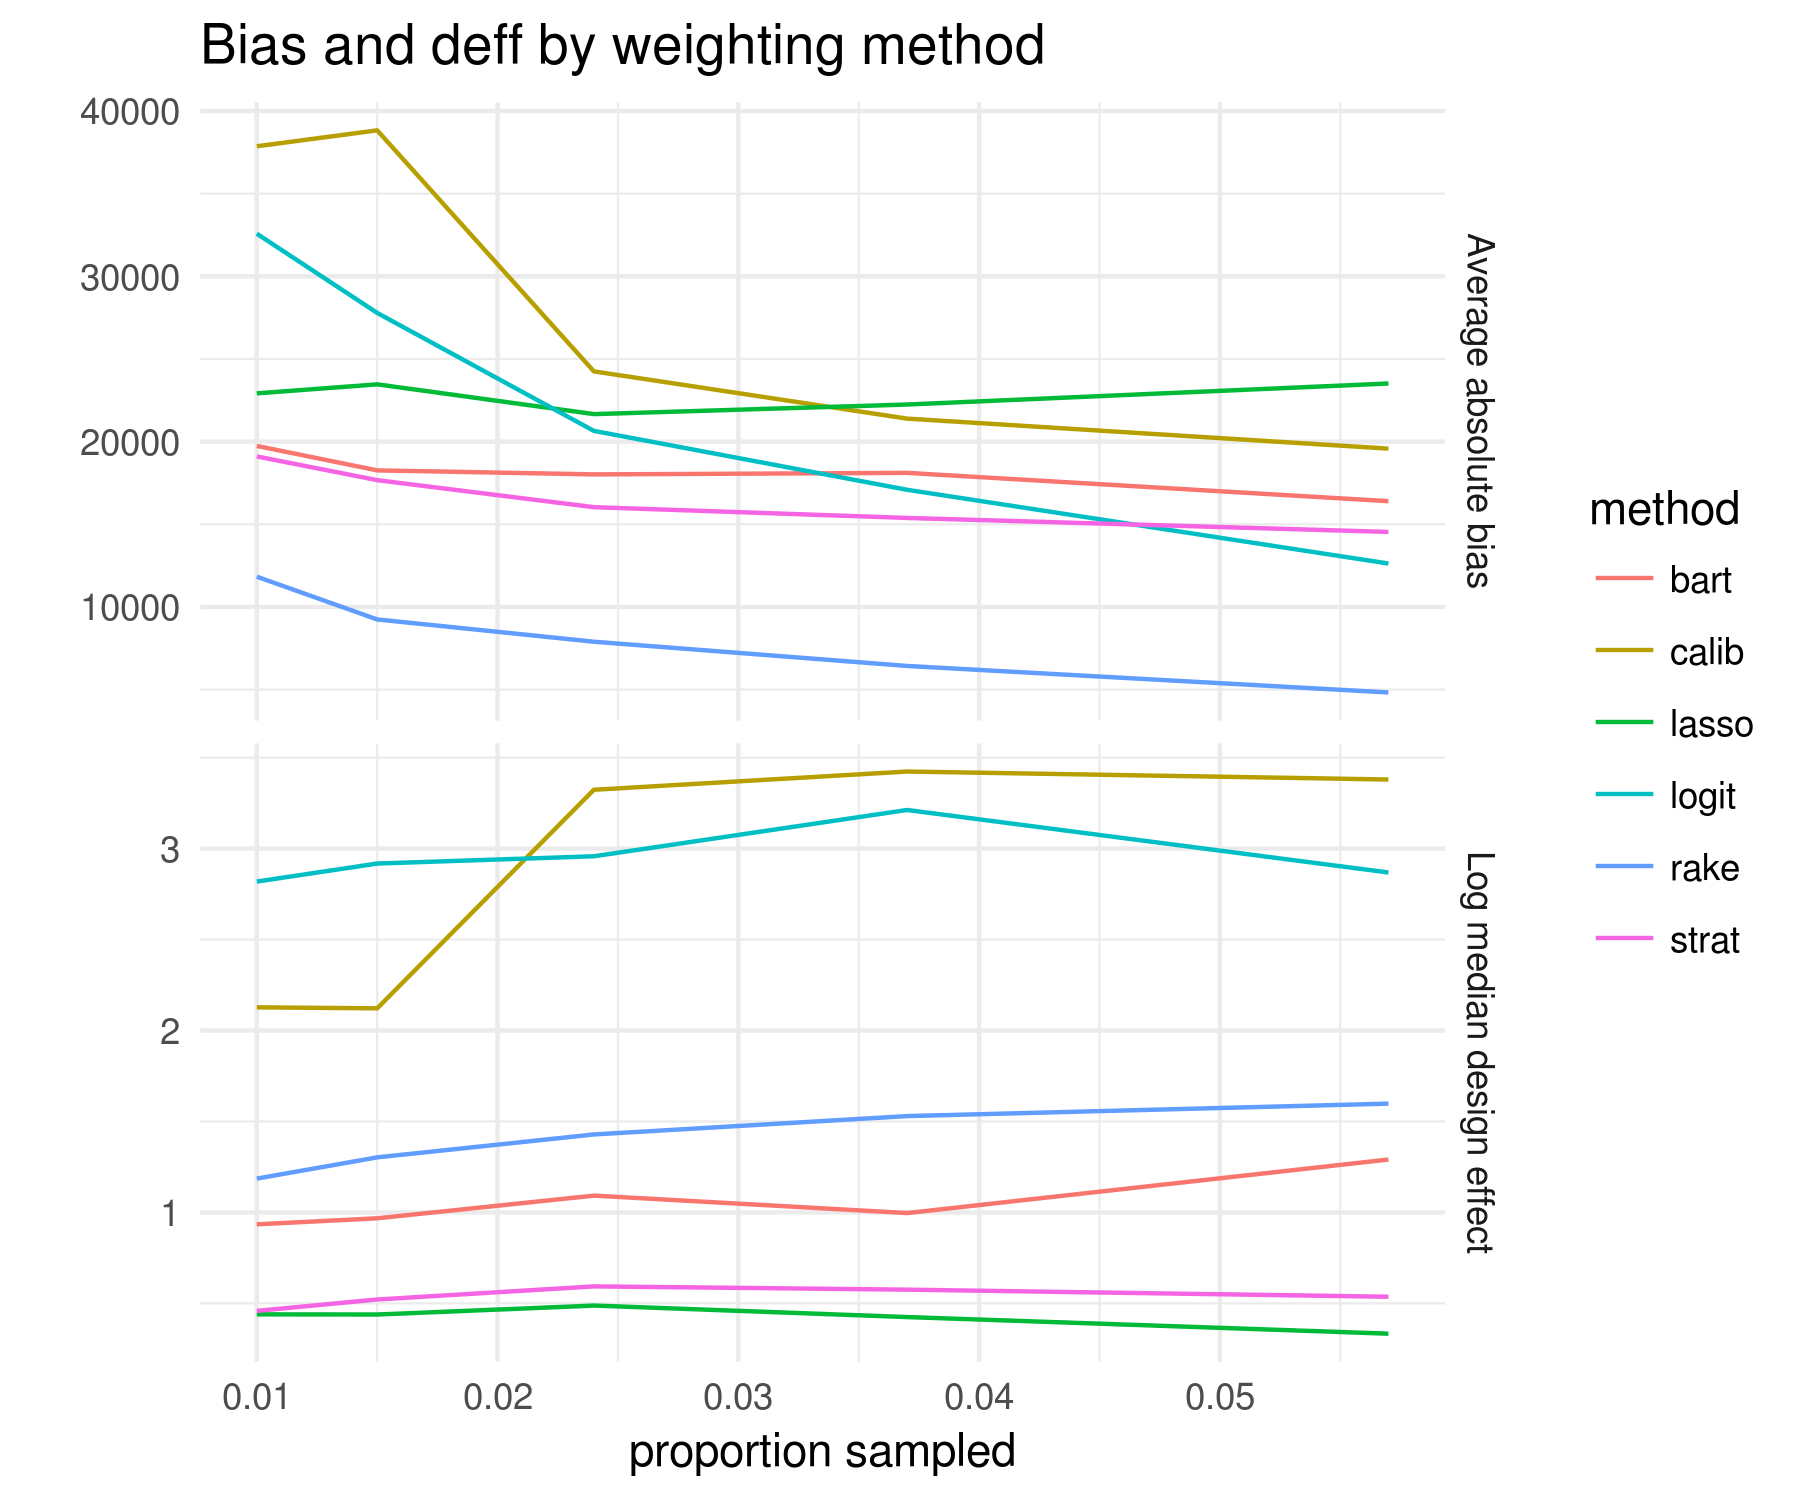
\includegraphics[width=0.75\textwidth]{~/github/mini-project-1/simulation/results/sim_1_5000_old_v3/plots/sim_results_presentation.png}
\end{figure}

\end{frame}

\begin{frame}{Simulation results - Remarks}
\protect\hypertarget{simulation-results---remarks}{}

\begin{itemize}
\tightlist
\item
  \emph{Post-stratification} performs surprisingly well, likely due to
  the size of the data set

  \begin{itemize}
  \tightlist
  \item
    note that stratification variables chosen with a random forest (not
    the standard implementation)
  \end{itemize}
\item
  \emph{BART + raking} outperforms other methods at the smallest sample
  sizes (which is probably the most realistic setting)
\item
  \emph{Calibration} performs very poorly - fails to correct bias and
  has large variance (likely from sensitivity to age distribution)
\item
  Directly predicting \(P(S = 1 | \mathbf{Z})\) with \emph{logistic
  regression} corrected bias well, but at a rather large cost in
  variance
\item
  \emph{LASSO} has smallest deff, but also fails to correct bias
  (variable selection not working well)
\end{itemize}

\end{frame}

\begin{frame}{Application to UK Biobank imaging cohort}
\protect\hypertarget{application-to-uk-biobank-imaging-cohort}{}

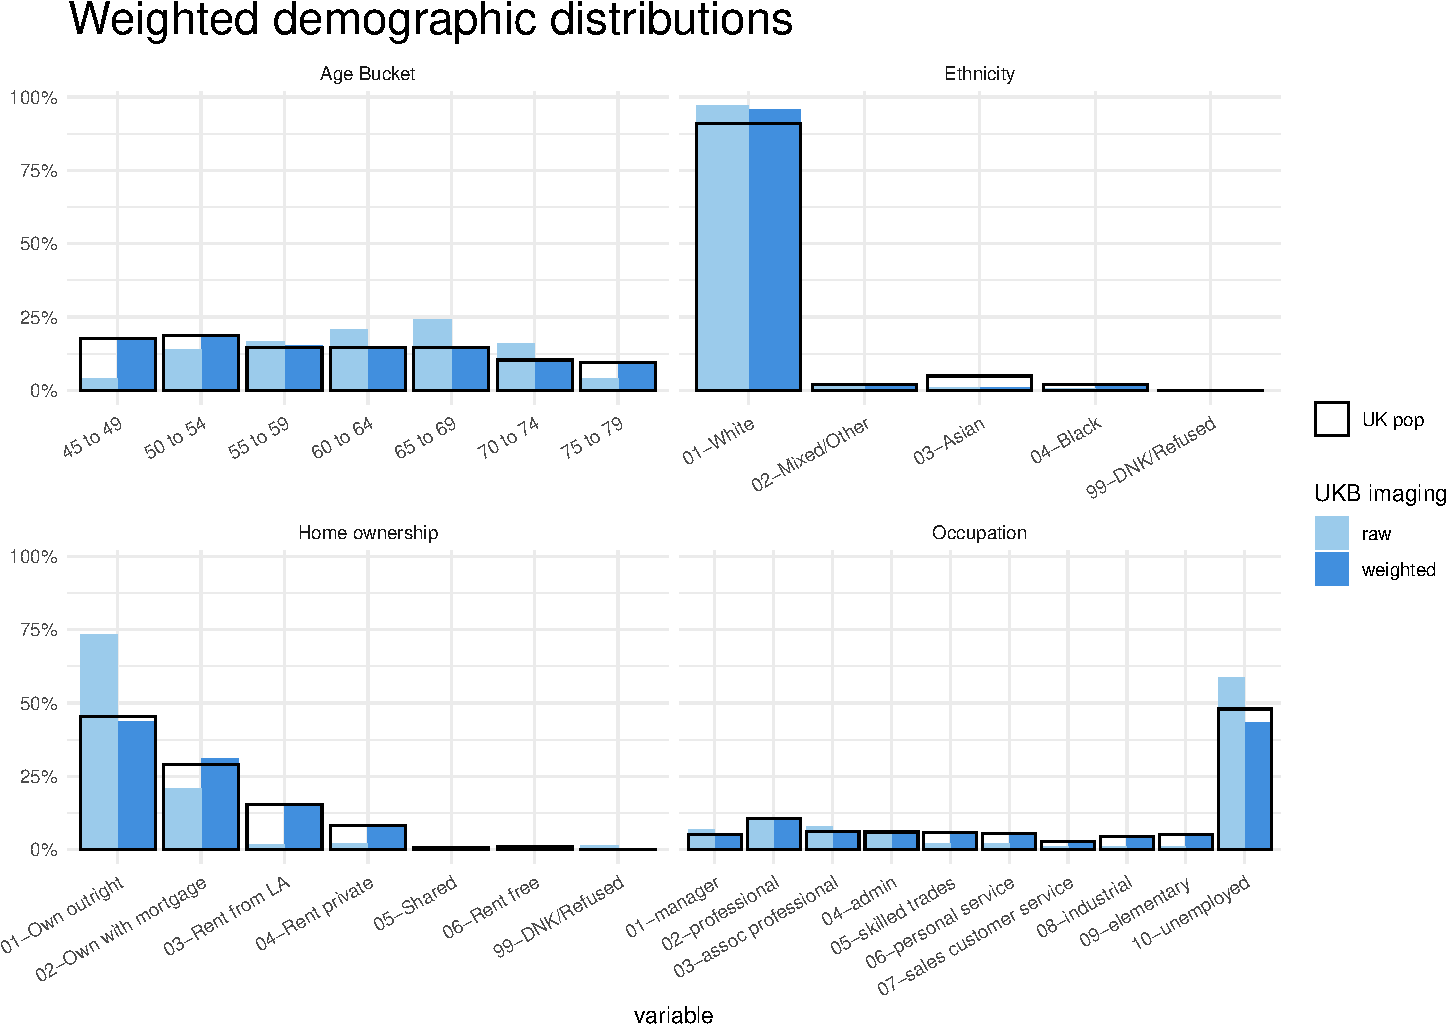
\includegraphics{fmrib-deck-20191002_files/figure-beamer/fig-ukb-results-demo-1.pdf}

\end{frame}

\begin{frame}{Application to UK Biobank imaging cohort}
\protect\hypertarget{application-to-uk-biobank-imaging-cohort-1}{}

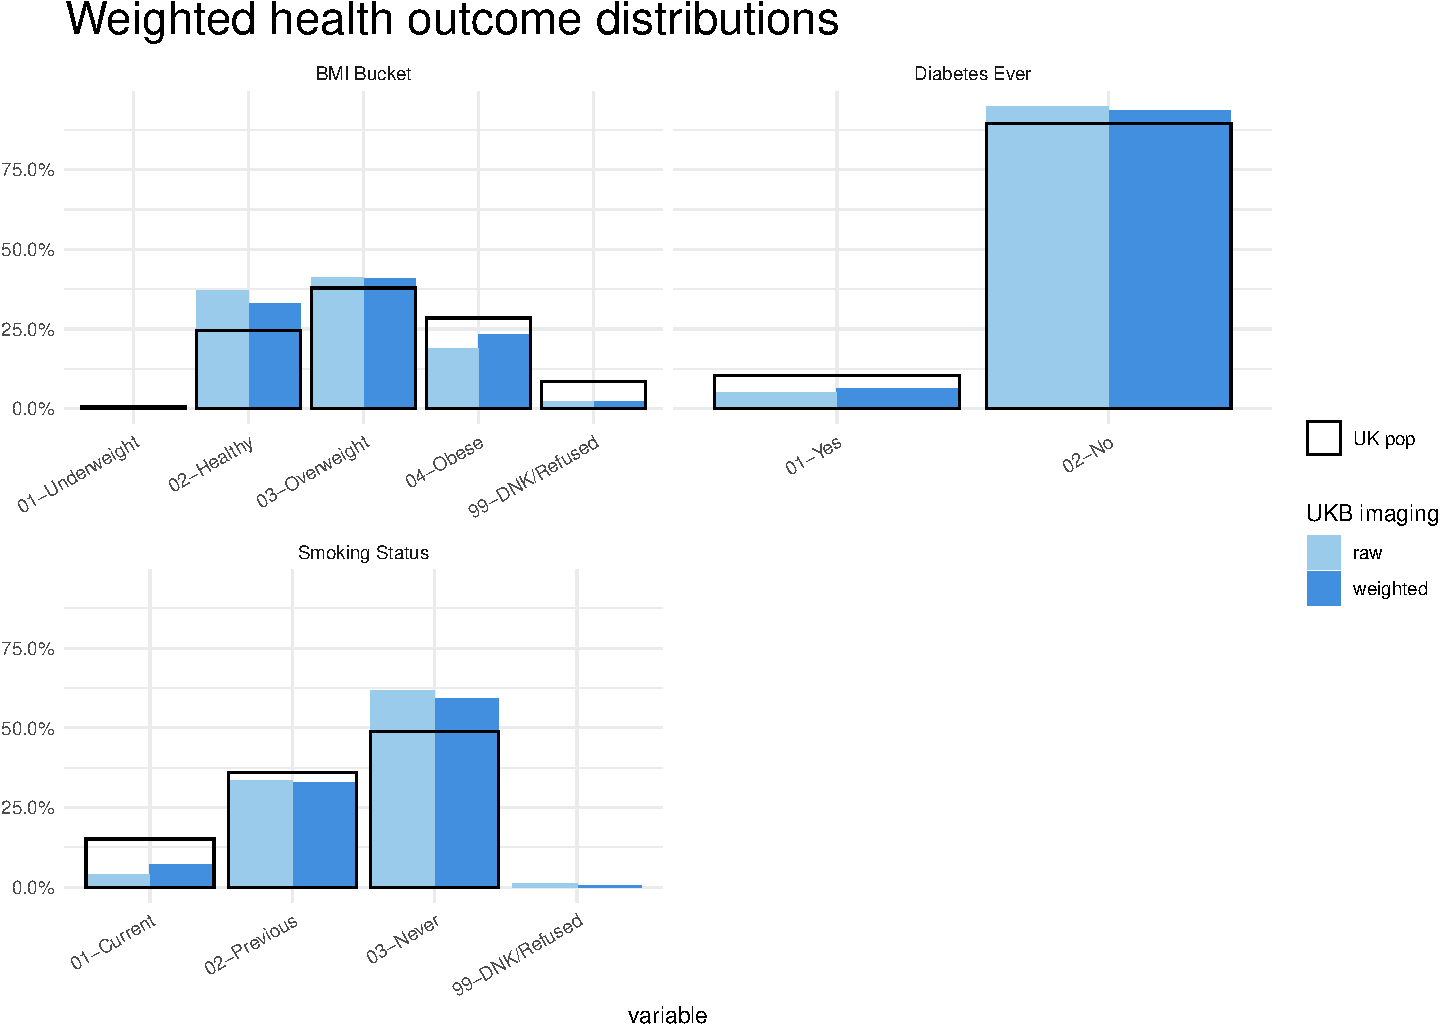
\includegraphics{fmrib-deck-20191002_files/figure-beamer/fig-ukb-results-health-1.pdf}

\end{frame}

\begin{frame}{Application to the UK Biobank imaging cohort}
\protect\hypertarget{application-to-the-uk-biobank-imaging-cohort}{}

\begin{figure}
\centering
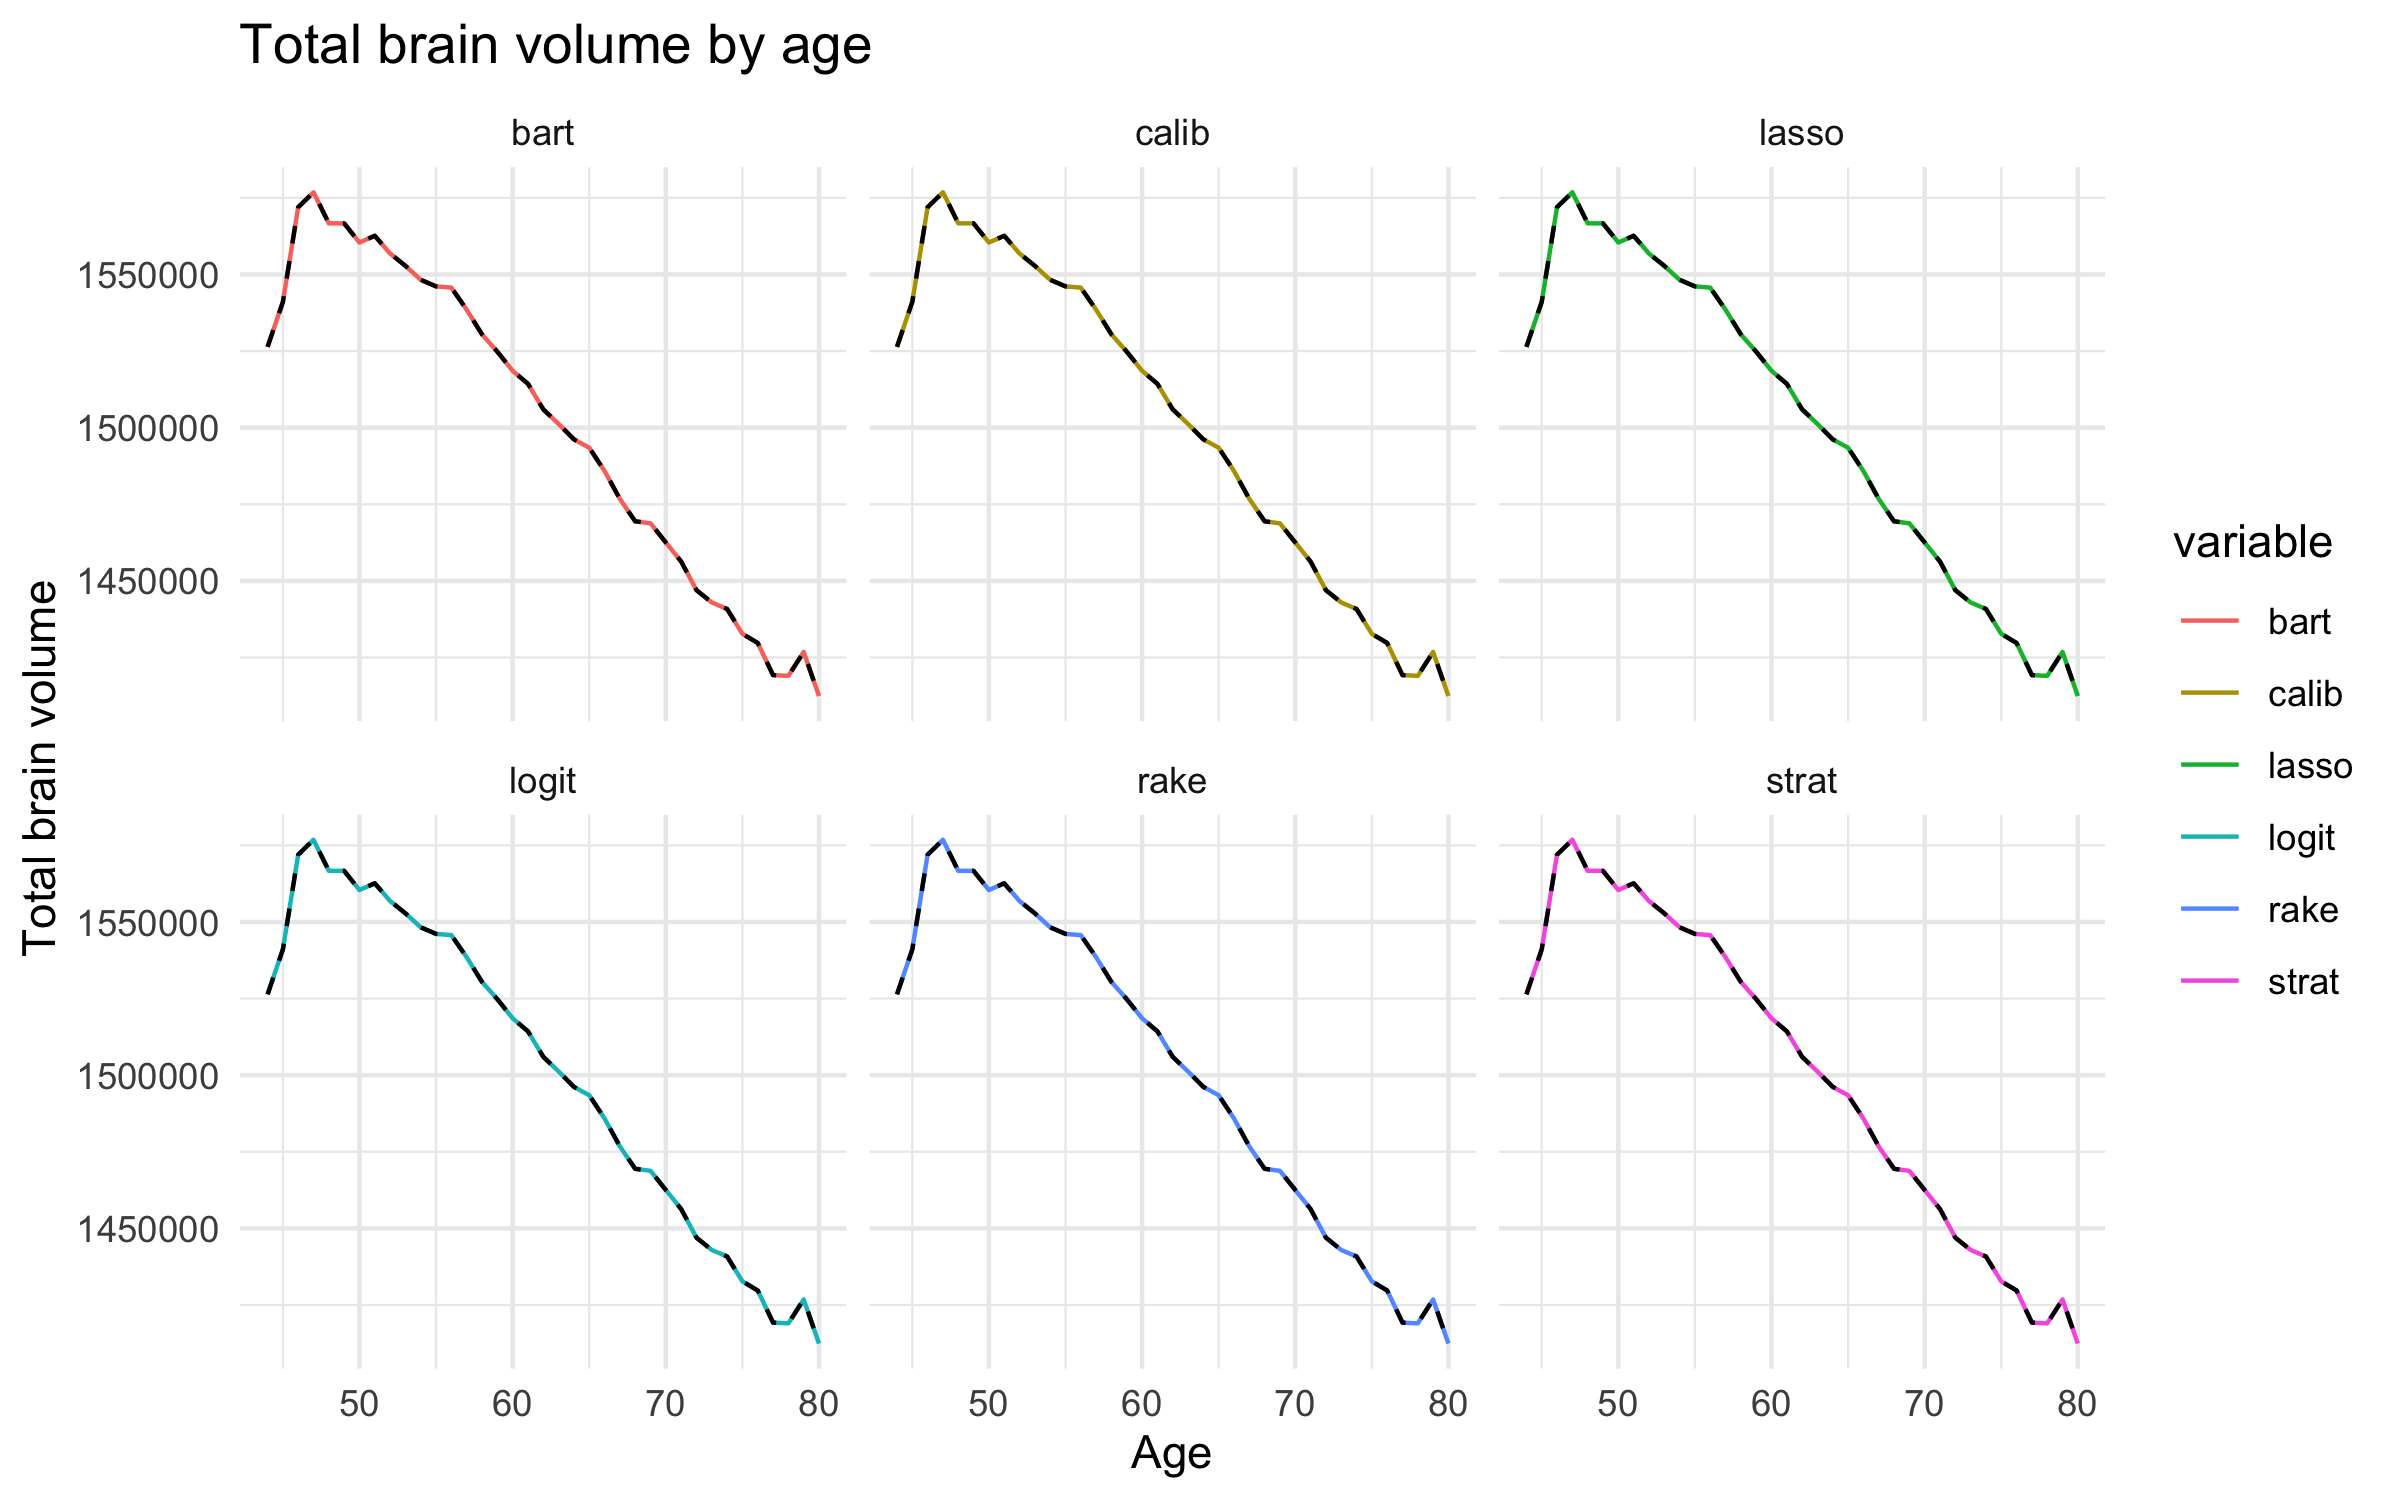
\includegraphics[width=\textwidth]{~/github/mini-project-1/simulation/results/sim_1_5000_old_v3/plots/ukb_brainvol_age.png}
\end{figure}

\end{frame}

\begin{frame}{Summary}
\protect\hypertarget{summary}{}

\begin{itemize}
\item
  Be wary of collider bias when estimating associations in the UK
  Biobank!
\item
  SCMs are a good framework for thinking about dependence structures,
  potential sources of bias, and if that bias can be corrected
\item
  \textbf{inverse probability weighting} can be used to adjust for
  selection bias, many different ways to estimate weights
\item
  Weighting the UKB imaging cohort corrects most of the bias in the
  demographic covariates, but only some of the bias in health outcomes
\end{itemize}

\end{frame}

\hypertarget{appendix}{%
\section{Appendix}\label{appendix}}

\begin{frame}{Method 1: Post-stratification}
\protect\hypertarget{method-1-post-stratification}{}

Adjust to the \emph{joint} distribution of \(\mathbf{Z}\). This is
exactly the definition for recovery (i.e.~a sum over all combinations of
levels of \(\mathbf{Z}\))

\begin{enumerate}
\tightlist
\item
  Define strata based on the full joint distribution of \(\mathbf{Z}\)
\item
  Calculate the probability of selection for each stratum
\item
  Apply stratum-level estimates to individuals
\end{enumerate}

Example:

\begin{table}[H]
\small
    \centering
    \begin{tabular}{|c c | c c |c | c|}
    \hline
    \textbf{sex} & \textbf{age} & \textbf{N (sample)} & \textbf{N (pop)} & $\hat{\text{P}}(S = 1 | \mathbf{Z}$) & $w^s$\\
    \hline
    Male & under 50 & 35 & 320 & $\frac{35}{320} = 0.109$ & $\frac{0.1}{0.109} = 0.917$\\
    Male & 50 plus & 11 & 133 & 0.083 & 1.20\\
    Female & under 50 & 41 & 355 & 0.115 & 0.870\\
    Female & 50 plus & 13 & 192 & 0.068 & 1.47\\
    \hline
    \end{tabular}
\end{table}

where \(\text{P}(S = 1) = 0.1\)

Then, all men under 50 in the study are given \(w^s = 0.917\)

\end{frame}

\begin{frame}{Method 1: Post-stratification}
\protect\hypertarget{method-1-post-stratification-1}{}

\textbf{Pros}:

\begin{itemize}
\tightlist
\item
  quick, closed-form solution
\item
  weighted joint distribution of \(\mathbf{Z}\) exactly matches that of
  the population
\end{itemize}

\textbf{Cons}:

\begin{itemize}
\tightlist
\item
  \(\mathbf{Z}\) must be discrete
\item
  can only consider a limited number of \(\mathbf{Z}\) before the strata
  get too small
\end{itemize}

\end{frame}

\begin{frame}{Method 2: Raking}
\protect\hypertarget{method-2-raking}{}

\emph{Iterative proportional fitting}; iteratively adjust the
\emph{marginal} distributions of auxilary variables \(\mathbf{Z}\)

\begin{enumerate}
\item
  Post-stratify to the population sex distribution
\item
  Post-stratify the \emph{weighted} sample to the population age
  distribution and update the weights
\item
  Post-stratify the \emph{new weighted} sample to the population sex
  distribution and update weights
\end{enumerate}

\ldots{}

Stop when weights stabilize (according to a tolerance threshold
\(\epsilon\))

\end{frame}

\begin{frame}{Method 2: Raking}
\protect\hypertarget{method-2-raking-1}{}

\textbf{Pros}:

\begin{itemize}
\tightlist
\item
  Weights are more stable, less extreme than post-stratification
\item
  Can consider a large set of variables \(\mathbf{Z}\)
\end{itemize}

\textbf{Cons}:

\begin{itemize}
\tightlist
\item
  Iterative (may never converge)
\item
  Not considering interactions between variables
\end{itemize}

(Basically the opposite of post-stratification)

\end{frame}

\begin{frame}{Method 3: Calibration}
\protect\hypertarget{method-3-calibration}{}

A generalization of raking that allows for continuous \(\mathbf{Z}\)

Instead of iterating over marginal distributions of elements in
\(\mathbf{Z}\) (i.e.~P(sex) and P(age)), we iterate over the totals of
each level of each element in \(\mathbf{Z}\) (i.e.~female, male, under
50, over 50).

With this formlation, we can also enforce constraints (weight) on
\textbf{continuous} variables. * e.g.~we constrain the mean age of the
sample

\emph{Con:} can be very finicky, even less likely to converge than
raking

\end{frame}

\begin{frame}{Method 4: Directly estimate
\(\hat{\text{P}}(S = 1| \mathbf{Z})\) with regression}
\protect\hypertarget{method-4-directly-estimate-hattextps-1-mathbfz-with-regression}{}

We use logistic regression to estimate
\(\hat{\text{P}}(S_i = 1 | \mathbf{Z}_i)\) because selection is binary
(S = 1 if observed, 0 otherwise):

\[\hat{\text{P}}(S_i = 1 | \mathbf{Z}_i) = \text{logit}^{-1}(\boldsymbol{\beta}\mathbf{Z}_i)\]

\textbf{Pros:}

\begin{itemize}
\tightlist
\item
  Can account for a large \(\mathbf{Z}\), including continous variables
  and interactions
\item
  Don't need custom weighting tools, just logistic regression
\end{itemize}

\textbf{Cons:}

\begin{itemize}
\tightlist
\item
  Weighted distribution of \(\mathbf{Z}\) will almost certainly not
  match population distributions (making results much less
  interpretable)
\item
  Requires individual-level population data
\end{itemize}

\end{frame}

\begin{frame}{Method 5: Raking with LASSO variable selection}
\protect\hypertarget{method-5-raking-with-lasso-variable-selection}{}

\textbf{Problem:} Both raking and post-stratification can fail when
\(\mathbf{Z}\) is too large

\textbf{Solution:} Select significant subsets of \(\mathbf{Z}\) using
LASSO, then rake to those marginals (Caughey and Hartman 2017)

General procedure:

\begin{enumerate}
\tightlist
\item
  Specify all levels of \(\mathbf{Z}\) and subsets to consider (i.e.~all
  first-order terms, and maybe two-way interactions)
\item
  Fit LASSO to
  \(S_i = \text{logit}^{-1}(\boldsymbol{\beta}\mathbf{Z}_i)\)
\item
  Fit LASSO to \(Y_i = f(\boldsymbol{\beta}\mathbf{Z}_i)\) (\(f\)
  depends on likelihood of \(Y\))
\item
  Rake to marginal distributions of all levels of \(\mathbf{Z}\) for
  which the corresponding \(\beta \neq 0\) in either of the LASSOs
\end{enumerate}

\textbf{Caution:} Highly dependent on LASSO performance

\end{frame}

\begin{frame}{Method 6: BART + raking}
\protect\hypertarget{method-6-bart-raking}{}

\textbf{Intuition:} Use \textbf{Bayesian additive regression tree
(BART)} to estimate \(P(S = 1 | \mathbf{Z})\), then rake to selected
\(\mathbf{Z}\) so that marginal distributions match (for
interpretability)

Why a BART?

\begin{itemize}
\tightlist
\item
  Trees are great for interactions
\item
  Some parallels to post-stratification
\end{itemize}

(but could use any method)

\textbf{Caution:} Computation time much greater than other methods

\end{frame}

\begin{frame}[allowframebreaks]{References}
\protect\hypertarget{references}{}

\small

\hypertarget{refs}{}
\leavevmode\hypertarget{ref-Caughey2017}{}%
Caughey, Devin, and Erin Hartman. 2017. ``Target Selection as Variable
Selection : Using the Lasso to Select Auxiliary Vectors for the
Construction of Survey Weights.''

\leavevmode\hypertarget{ref-Correa2018}{}%
Correa, J D, J Tian, and E Bareinboim. 2018. ``Generalized adjustment
under confounding and selection biases.'' \emph{32nd AAAI Conference on
Artificial Intelligence, AAAI 2018}, no. June: 6335--42.
\url{https://www.aaai.org/ocs/index.php/AAAI/AAAI18/paper/viewFile/17375/16207}.

\leavevmode\hypertarget{ref-Day2016}{}%
Day, Felix R., Po Ru Loh, Robert A. Scott, Ken K. Ong, and John R. B.
Perry. 2016. ``A Robust Example of Collider Bias in a Genetic
Association Study.'' \emph{American Journal of Human Genetics} 98 (2):
392--93. \url{https://doi.org/10.1016/j.ajhg.2015.12.019}.

\leavevmode\hypertarget{ref-fry2017comparison}{}%
Fry, Anna, Thomas J Littlejohns, Cathie Sudlow, Nicola Doherty, Ligia
Adamska, Tim Sprosen, Rory Collins, and Naomi E Allen. 2017.
``Comparison of Sociodemographic and Health-Related Characteristics of
Uk Biobank Participants with Those of the General Population.''
\emph{American Journal of Epidemiology} 186 (9): 1026--34.

\leavevmode\hypertarget{ref-Munafo2018}{}%
Munafò, Marcus R., Kate Tilling, Amy E. Taylor, David M. Evans, and
George Davey Smith. 2018. ``Collider scope: When selection bias can
substantially influence observed associations.'' \emph{International
Journal of Epidemiology} 47 (1): 226--35.
\url{https://doi.org/10.1093/ije/dyx206}.

\leavevmode\hypertarget{ref-Pearl1995}{}%
Pearl, Judea. 1995. ``Causal diagrams for empirical research.''
\emph{Biometrika} 82 (4): 669--710.
\url{https://doi.org/10.1093/biomet/82.4.700}.

\end{frame}

\end{document}
